\chapter{Podsumowanie}


\section{Zdjęcia implementacji}

Jak pokazano na rys.~\ref{fig:arduino_schowek} mikrokontroler znajduje w schowku przed fotelem pasażera. Wyświetlacz wraz z przyciskiem został osadzony przy kierownicy. (rys.~\ref{fig:arduino_lcd}).

\begin{figure}[!htb]
\centering
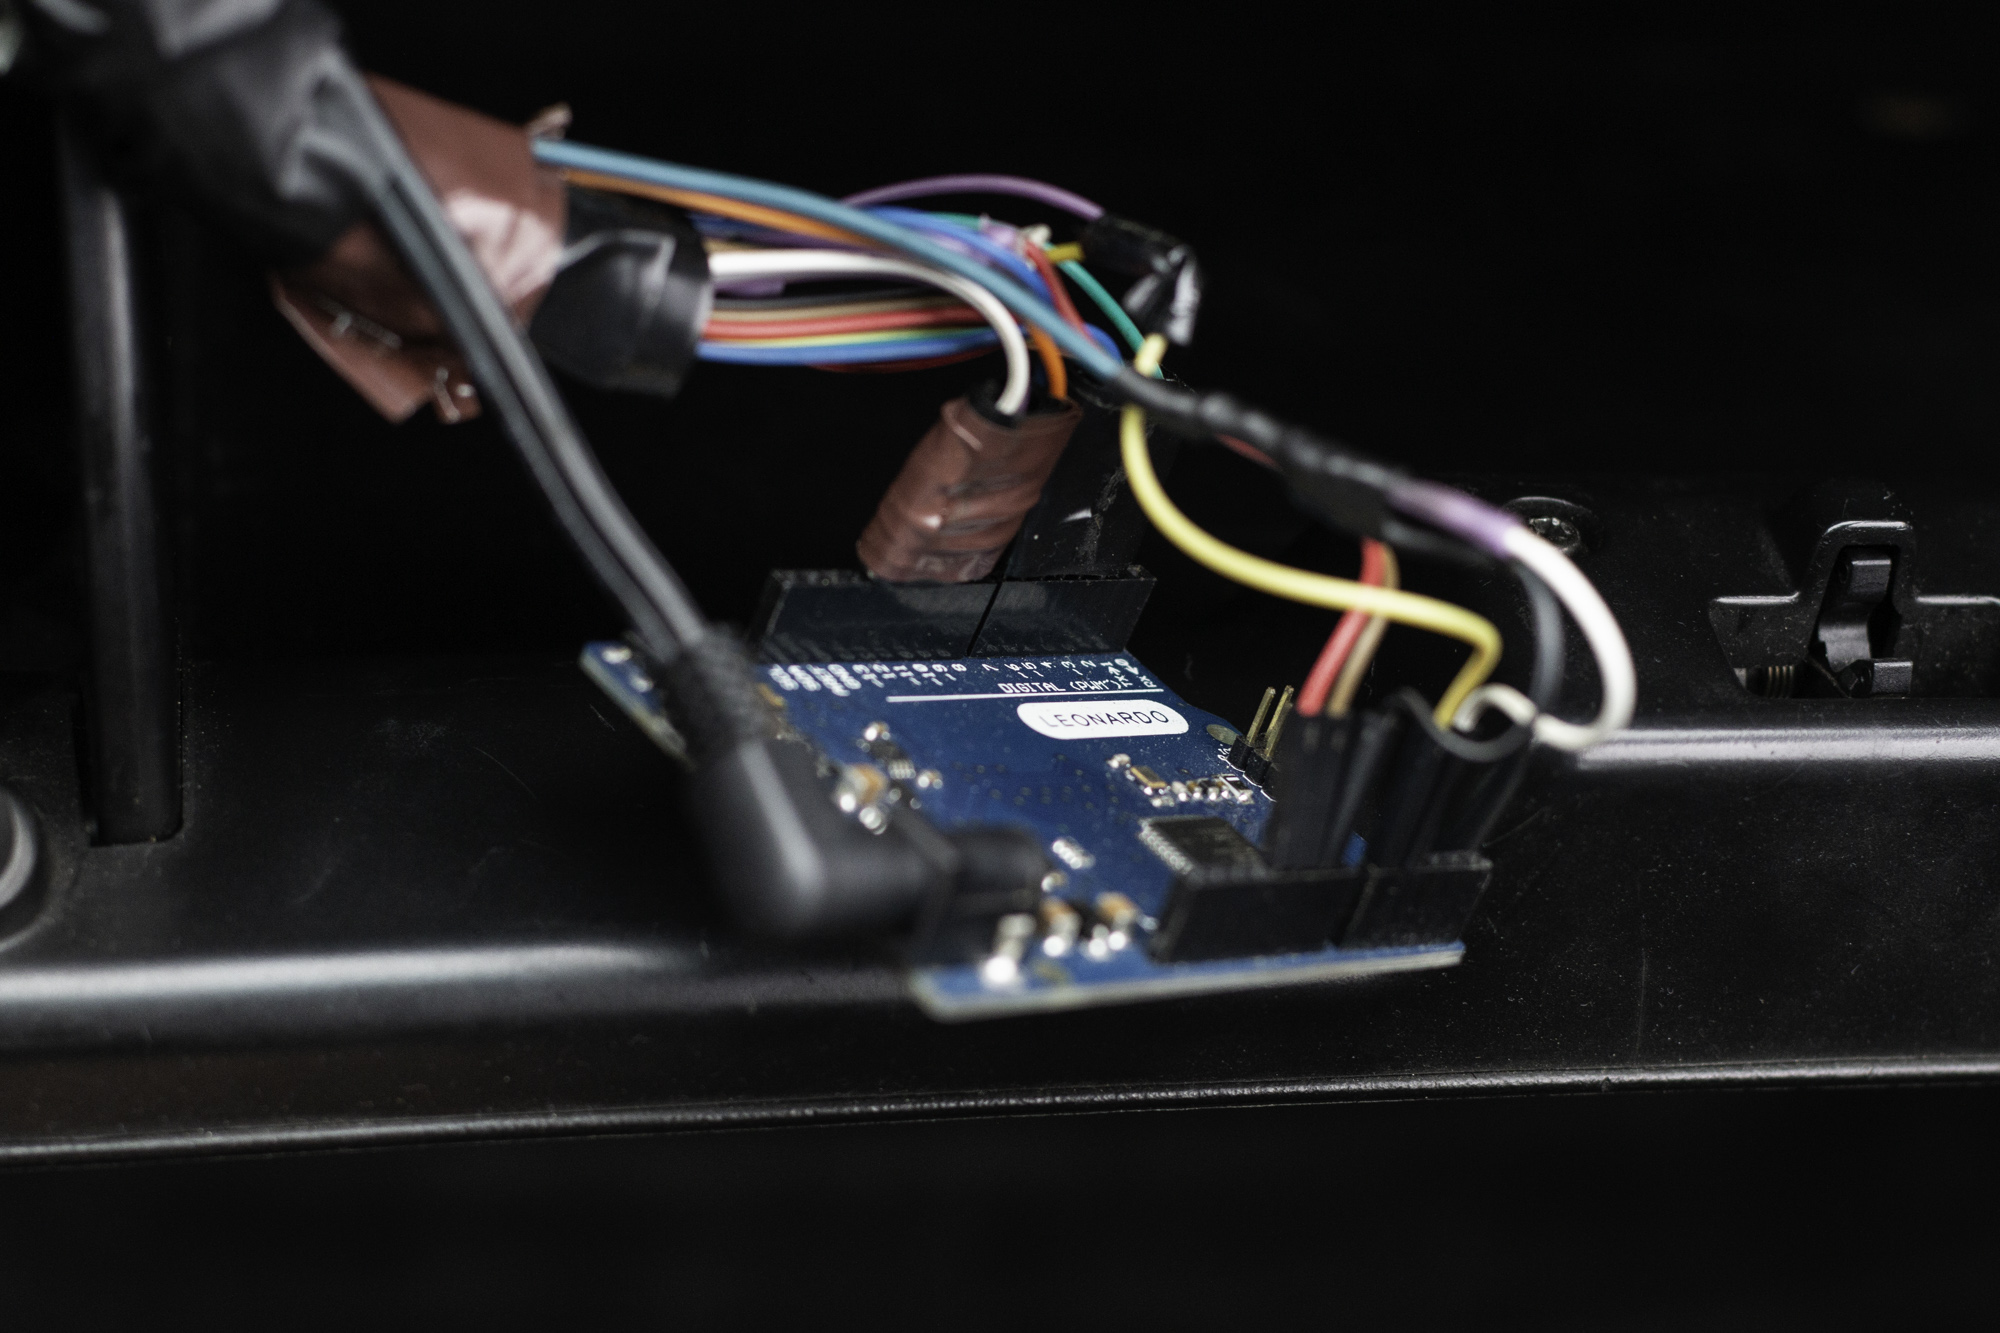
\includegraphics[width=0.8\linewidth]{Rysunki/arduino_schowek.jpg}
\caption{Mikrokontroler w schowku}
\label{fig:arduino_schowek}
\end{figure}
\begin{figure}[!htb]
\centering
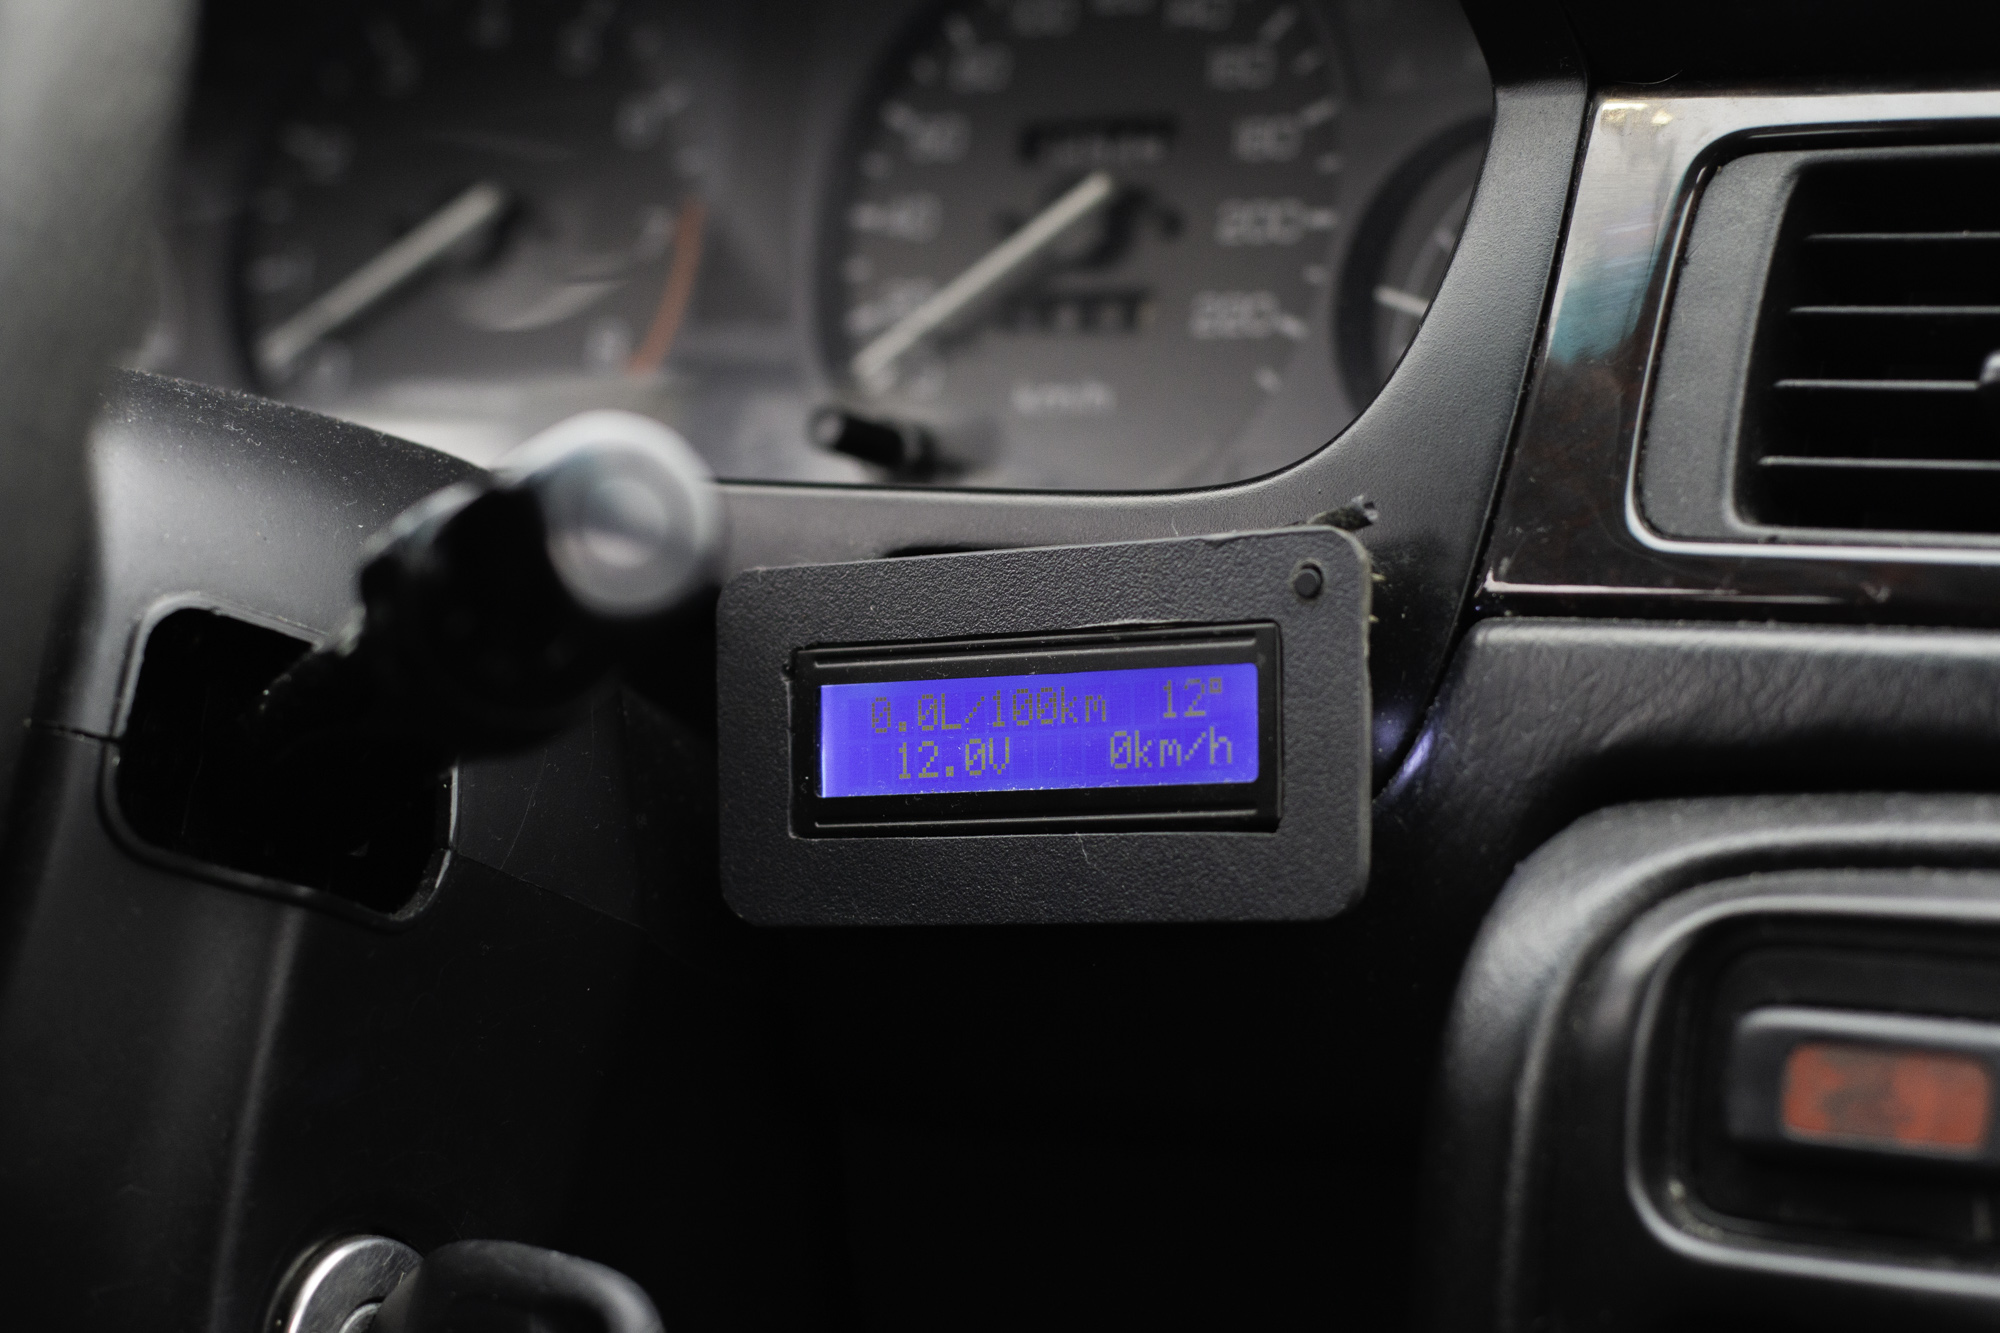
\includegraphics[width=0.8\linewidth]{Rysunki/arduino_lcd.jpg}
\caption{Miejsce osadzenia wyświetlacza}
\label{fig:arduino_lcd}
\end{figure}


\section{Wykonane prace}
Podsumowując, w ramach tej pracy została stworzona implementacja mikrokontrolera, który oblicza i wyświetla informacje o aktualnym stanie pojazdu, tj. informacje na temat spalania, prędkości, temperatury, napięciu w układzie samochodu oraz aktualnego położenia pedału gazu. Ze względu na swoją uniwersalność projekt ten można zastosować do pojazdów różnych marek.
\section{Możliwości rozbudowy}
Jako, iż projekt jest oparty o platformę Arduino można go dalej rozbudowywać rozbudować. Niektórymi z możliwości dalszej rozbudowy są:
\begin{itemize}
\item dodanie modułu bezprzewodowego (Bluetooth/ Wi-Fi) do synchronizacji danych,
\item dodanie modułu GPS do zapisu tras,
\item dodanie modułu GSM, który w połączeniu z systemem GPS mógłby służyć jako system antykradzieżowy do lokalizacji pojazdu,
\item zastosowanie magistrali I2C, aby zredukować ilość zajętych pinów i komunikować się po niej z zewnętrznymi modułami (LCD, GSM, GPS itp.)
\item jako, iż aktualne informacje o położeniu pedału gazu nie są potrzebne do żadnych obliczeń, są tylko wyświetlane na ekranie, można wykorzystać je do zaawansowanych statystyk na temat spalania oraz skonstruować funkcjonalność, która pomagałaby redukować spalanie poprzez informacje jakie położenie pedału gazu w danym momencie jest najbardziej optymalne.
\item można podłączyć czujniki zbliżeniowe, które służyłyby jako czujniki parkowania, moduł mógłby wtedy graficznie informować o przeszkodach wokół samochodu.
\end{itemize}
